\section{Methodology}

\subsection{N-Dimension Matrix}
\begin{frame}
  \frametitle{N-dimension Matrix}
  \framesubtitle{Challanges}
  STL provides containers \texttt{std::array} and \texttt{std::vector} for creating one-dimension array.
  \\
  There are two way for dealing with high-dimension data:
  \begin{enumerate}
    \item Nesting the one dimension arrays or vectors.
    \item Hierarchy approach, designing derived classes of one-dimension array base class.
  \end{enumerate}
  \begin{figure}[htbp]
    \centering
    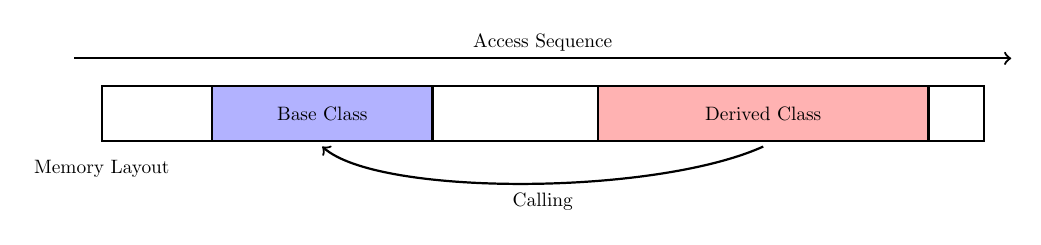
\begin{tikzpicture}[scale=0.7, transform shape]
      % \draw[help lines, step=1] (-10,-2) grid (10,2);    
      % % Draw axes
      % \draw[dashed,->] (-10,0) -- (10,0) node[right] {x};
      % \draw[dashed,->] (0,-2) -- (0,2) node[above] {y};

      \draw[thick, ->] (-8.5, 1.5) -- node[midway, above] {Access Sequence} (8.5, 1.5);

      \draw[thick] (-8,1) rectangle (8,0);
      \node at (-8,-0.5) [] {Memory Layout};

      \draw[thick, fill=blue!30] (-6,1) rectangle (-2,0);
      \node at (-4, 0.5) [] {Base Class};

      \draw[thick, fill=red!30] (1,1) rectangle (7,0);
      \node at (4, 0.5) [] {Derived Class};

      \node at (0, -1.1) [] {Calling};
      \draw[thick, ->] (4, -0.1) 
        .. controls (2, -1) and (-3, -1) .. (-4, -0.1);

    \end{tikzpicture}
    \caption{Derived Class calling members in Base class, timing is not predictable.}
    \label{<label>}
  \end{figure}
\end{frame}


\begin{frame}
  % \frametitle{N-dimension Matrix}
  % \framesubtitle{Memory Layout Problem}
  \begin{enumerate}
    \item Nesting multi-dimension array has non-contiguous memory layout.
    \item Derived class needs more time to access members in base class.
    \item Poor cache utilization leads to poor performance.
    \item MPI type create requires contiguous memory layout.
  \end{enumerate}
  % 插入图
  \begin{figure}[htbp]
    \centering
    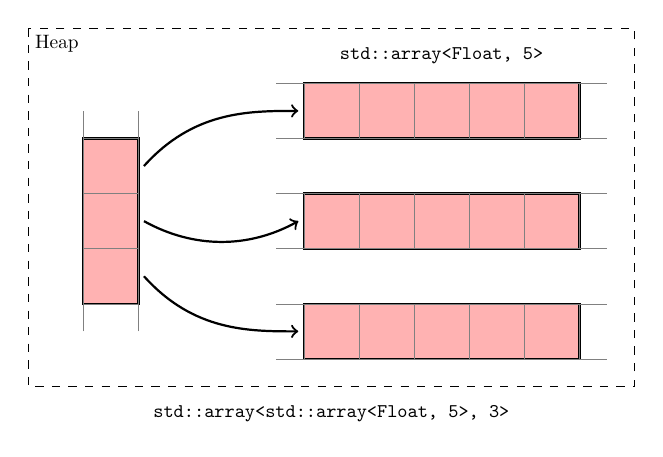
\begin{tikzpicture}[scale=0.7, transform shape]
      % \draw[help lines, step=1] (-10,-2) grid (10,2);    
      % Draw axes
      % \draw[dashed,->] (-10,0) -- (10,0) node[right] {x};
      % \draw[dashed,->] (0,-2) -- (0,2) node[above] {y};

      \draw[dashed] (-1, 3) rectangle (10, -3.5);
      \node at (-1, 3) [below right] {Heap}; 
      
      \node at (4.5, -4) [] {\texttt{std::array<std::array<Float, 5>, 3>}};
      \node at (6.5, 2.5) [] {\texttt{std::array<Float, 5>}};


      \draw[thick, fill=red!30] (0, 1) rectangle (1, -2);
      \draw[help lines, step=1] (0,1.5) grid (1,-2.5);


      \draw[thick, fill=red!30] (4, 2) rectangle (9, 1);
      \draw[help lines, step=1] (3.5, 2) grid (9.5, 1);
      
      \draw[thick, fill=red!30] (4, 0) rectangle (9, -1);
      \draw[help lines, step=1] (3.5, 0) grid (9.5, -1);
      

      \draw[thick, fill=red!30] (4, -2) rectangle (9, -3);
      \draw[help lines, step=1] (3.5,-2) grid (9.5,-3);


      \draw[thick, ->] (1.1, 0.5) 
      .. controls (2, 1.5) and (3, 1.5) .. (3.9, 1.5);

      \draw[thick, ->] (1.1, -0.5) 
      .. controls (2, -1) and (3, -1) .. (3.9, -0.5);

      \draw[thick, ->] (1.1, -1.5) 
      .. controls (2, -2.5) and (3, -2.5) .. (3.9, -2.5);
      
    \end{tikzpicture}
    \caption{Using nested \texttt{std::array<T, N>} to store 2D array data.}
    \label{<label>}
  \end{figure}
\end{frame}


\begin{frame}
  \frametitle{N-dimension Matrix}
  \framesubtitle{Solution}
  \begin{itemize}
    \item Separate into two detail and user interface objects adhering RAII rules.
    \steporfull<2->{
      \item An external small \texttt{\_\_multi\_array\_shape} object defines the routines for accessing the elements.
    }
    \steporfull<3->{
      \item Smart pointer, ensure memory's contiguous layout and safety.
    }
  \end{itemize}


  \begin{figure}[htbp]
    \centering
    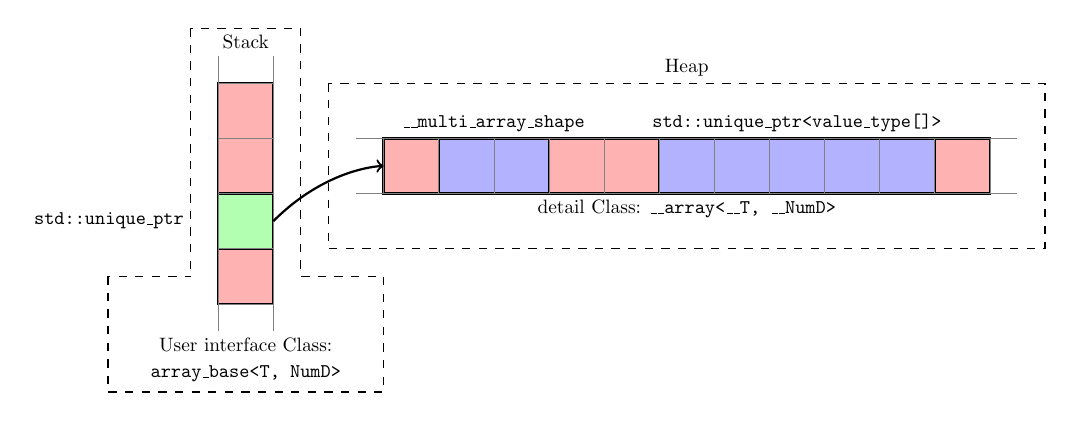
\begin{tikzpicture}[scale=0.7, transform shape]
      % \draw[help lines, step=1] (-10,-2) grid (10,2);    
      % % Draw axes
      % \draw[dashed,->] (-10,0) -- (10,0) node[right] {x};
      % \draw[dashed,->] (0,-2) -- (0,2) node[above] {y};      
  
      \draw[dashed] (-2, 2) rectangle (11, -1);
      \node at (4.5, 2) [above] {Heap}; 

      \draw[thick, fill=red!30] (-1, 1) rectangle (10, 0);
      \node at (4.5, 0) [below] {detail Class: \texttt{\_\_array<\_\_T, \_\_NumD>}};

      \steporfull<2->{
        \draw[thick, fill=blue!30] (0, 1) rectangle (2, 0);
        \node at (1, 1) [above] {\texttt{\_\_multi\_array\_shape}};
        \draw[thick, fill=blue!30] (4, 1) rectangle (9, 0);
        \node at (6.5,1) [above] {\texttt{std::unique\_ptr<value\_type[]>}}; 
      }
      \draw[help lines, step=1] (-1.5, 1) grid (10.5, 0);    

      
      
      
      \node at (-3.5, 3) [below] {Stack}; 
      \draw[dashed] (-4.5, 3) rectangle (-2.5, -3);
      \draw[dashed, fill=white] (-6, -1.5) rectangle (-1, -3.6);

      \draw[draw=none, fill=white] (-4.5, -1.9) rectangle (-2.5, -2.1);
      \draw[draw=none, fill=white] (-4.5, -1.45) rectangle (-2.5, -1.55);



      \draw[thick, fill=red!30] (-4, 2) rectangle (-3, -2);

      \steporfull<3->{
        \draw[thick, fill=green!30] (-4, 0) rectangle (-3, -1);
        \node at (-4.5, -0.5) [left] {\texttt{std::unique\_ptr}}; 
      }
      \draw[help lines, step=1] (-4, 2.5) grid (-3, -2.5);    


      


      \node at (-3.5, -2.5) [below] {User interface Class:};
      \node at (-3.5, -3) [below] {\texttt{array\_base<T, NumD>}};
      \steporfull<3->{
        \draw[thick, ->] (-3, -0.5) 
          .. controls (-2, 0.5) and (-1, 0.5) .. (-1, 0.5);
      }
      

    \end{tikzpicture}

    \captionsetup{width=0.8\textwidth}
    \caption{
      The solution of N-dimension Matrix, using detail Class, user interface Class \steporfull<2->{and a shape management structure.}
    }
    \label{<label>}
  \end{figure}
\end{frame}







\subsection{Parallelization of N-dimension Arrays}
\begin{frame}
  \frametitle{Parallelization of N-dimension Arrays}
  \framesubtitle{MPI Environment}
  \hspace*{1em}The hybrid PDE solver requires the MPI supports multi-threads on each processes.\vspace*{1em}
  \begin{itemize}
    \item High-level libraries like Boost.MPI  
    \begin{enumerate}
      \item have better MPI resource management and other basic communication features.
      \item only provide limited useful features for latter PDE solvers.
      \item lead to lower performance than low-level OpenMPI. \vspace*{1em}
    \end{enumerate}
    \steporfull<2->{
      \item I developed an environment class for MPI 
      \begin{enumerate}
        \item better resource management than raw MPI.
        \item provides basic features exclusively for this project.
      \end{enumerate}
    }
  \end{itemize}
  
  \vspace*{1em}\hspace*{1em}

  % Creating an environment class for MPI resource management and provides basic features.

  % Ghost communication is required in overlapping of MPI communication and local computation.
  % Implementing distributions on class derived from N-dimension array class downgrades performance.

\end{frame}


\begin{frame}
  \frametitle{Parallelization of N-dimension Arrays}
  \framesubtitle{MPI Topology - Challanges}
  
  Distributed N-dimension arrays are created based on MPI N-dimension Cartesian topology.
  \steporfull<2->{
    \begin{enumerate}
      \item Ghost communication is required in overlapping of MPI communication and local computation.
      \item Parallel I/O is needed for debugging and storing results.
      \item Topology information will be frequently used in PDE solver.
    \end{enumerate}
  }
\end{frame}


\begin{frame}
  \frametitle{Parallelization of N-dimension Arrays}
  \framesubtitle{MPI Topology - Solution}
  \begin{enumerate}
    \item An MPI Topology class defines the distribution details of N-dimension array.
  \end{enumerate}
  \begin{figure}[htbp]
    \centering
    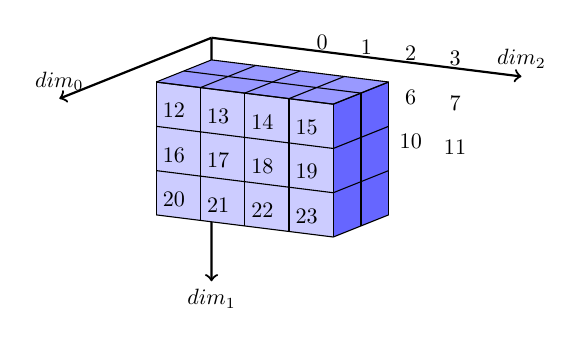
\begin{tikzpicture}[scale=0.8, transform shape]
      % \draw[help lines, step=1em] (0,0) grid (12em, 10em);
      % \draw[dashed, ->] (0,0) -- (12em, 0) node[right] {$x$};
      % \draw[dashed, ->] (0,0) -- (0, 10em) node[above] {$y$};
      
      \def\xsize{2};
      \def\ysize{3};
      \def\zsize{4};
    
      \begin{scope}[shift={(0em, 0em)}, x={(2em,-0.25em)},y={(0em,2em)}, , z={(-1.25em,-0.5em)}]
      % \draw[help lines, step=1em] (0,0,0) grid (0.5em, 0.5em, 0);
      \draw[thick, ->] (0,3.5,-0.2em) -- (7, 3.5, -2) node[above] {$dim_2$};
      \draw[thick, ->] (0,3.5,-0.2em) -- (0, -2, -2) node[below] {$dim_1$};
      \draw[thick, ->] (0,3.5,-0.2em) -- (0, 3.5, 3.5) node[above] {$dim_0$};
  
    \foreach \y in {0, 1, ..., \ysize}
    {
      \node at (\y/\ysize * \ysize,0.4 + \xsize, -6) {$\y$};
  
      \pgfmathsetmacro{\pid}{int(\y + \zsize)}
      \node at (\y/\ysize * \ysize,0.4 + \xsize - 1, -6) {$\pid$};
  
      \pgfmathsetmacro{\pidd}{int(\y + 2 * \zsize)}
      \node at (\y/\ysize * \ysize,0.4 + \xsize - 2, -6) {$\pidd$};
    }
        
        % Draw the front face
        \fill[blue!20] (0,0,0) -- (0,\ysize,0) -- (\zsize, \ysize,0) -- (\zsize,0,0) -- cycle;
        % Draw the top face
        \fill[blue!40] (0,\ysize,0) -- (0,\ysize,-\xsize) -- (\zsize, \ysize, -\xsize) -- (\zsize, \ysize,0) -- cycle;
        % Draw the right face
        \fill[blue!60] (\zsize,0,0) -- (\zsize,0,-\xsize) -- (\zsize, \ysize, -\xsize) -- (\zsize, \ysize,0) -- cycle;
  
    
        \foreach \x in {0,1, ..., \xsize}
        {
          \draw[black] (0, \ysize, -\x/\xsize * \xsize) -- (\zsize, \ysize, -\x/\xsize * \xsize);
          \draw[black] (\zsize,0,-\x/\xsize * \xsize) -- (\zsize, \ysize,-\x/\xsize * \xsize);
        }
    
        \foreach \y in {0, 1, ..., \ysize}
        {
          \draw[black] (0,\y/\ysize * \ysize,0) -- (\zsize,\y/\ysize * \ysize,0);
          \draw[black] (\zsize,\y/\ysize * \ysize,0) -- (\zsize,\y/\ysize * \ysize,-\xsize);
        }
    
        \foreach \z in {0, 1, ..., \zsize}
        {
          \draw[black] (\z/\zsize * \zsize,\ysize,0) -- (\z/\zsize * \zsize,\ysize,-\xsize);
          \draw[black] (\z/\zsize * \zsize,0,0) -- (\z/\zsize * \zsize,\ysize,0);
        }
  
        \foreach \y in {0, 1, ..., \ysize}
        {
          \pgfmathsetmacro{\pid}{int(\y + 12)}
          \node at (\y/\ysize * \ysize + 0.4,0.4 + \xsize, 0) {$\pid$};
  
          \pgfmathsetmacro{\pidd}{int(\y + \zsize + 12)}
          \node at (\y/\ysize * \ysize + 0.4,0.4 + \xsize - 1, 0) {$\pidd$};
  
          \pgfmathsetmacro{\piddd}{int(\y + 2 * \zsize + 12)}
          \node at (\y/\ysize * \ysize + 0.4,0.4 + \xsize - 2, 0) {$\piddd$};
        }
      \end{scope}
    \end{tikzpicture}
    \caption{
          The Schematic representation of the MPI Cartesian topology scheme of $24$ processors on $3$ dimension space, 
          which has a $2\times 3\times 4$ grid of processes 
      }
    \label{FIG_MPI_TOPOLOGY_24_PROCS}
  \end{figure}
\end{frame}


\begin{frame}
  \frametitle{Parallelization of N-dimension Arrays}
  \framesubtitle{MPI Topology - Solution}
  \begin{enumerate}
    \setcounter{enumi}{1}
    \item Using \texttt{MPI\_Type\_create\_subarray} for creating Ghost MPI datatype for communication.
  \end{enumerate}

  \begin{figure}[htbp]
    \centering
    \begin{tikzpicture}[scale=0.8, transform shape]
      % Draw a grid with steps of 1 cm
      % \draw[help lines, step=1em] (-2em,-2em) grid (20em,20em);
    
      % Draw axes
      % \draw[dashed,->] (-2em,0) -- (20em,0) node[right] {x};
      % \draw[dashed,->] (0,-2em) -- (0,20em) node[above] {y};
    
      % Draw the first cube at (0,0) with size 8
      \drawcube{(0em, 0em)}{8}
      \drawcube{(16em, 0em)}{8}

    \end{tikzpicture}  
    \caption{
      Representation of a 3D MPI Communication Scheme of $2$ among $24$ processes between $3$ dimension sub-arrays.
    }
    \label{FIG_MPI_3D_exchange_SCHEME}
  \end{figure}


\end{frame}





\begin{frame}
  \frametitle{Parallelization of N-dimension Arrays}
  \framesubtitle{MPI Topology - Solution}
  \begin{enumerate}
    \setcounter{enumi}{2}
    \item Cartesian array has members Topology class and N-dimension array class, to ensure they are closely located on memory.
    \item The external functions provide gather-based I/O and MPI I/O for handling different scenarios.
    \begin{itemize}
      \item gather-based function is designed for small scale problem, \\it collects all data included with the boundaries to the root process, and use the I/O of N-dimension array.
      \item MPI I/O function is designed for handling large scale problem, \\it only collects the internal bulk without boundary.
    \end{itemize}
  \end{enumerate}
\end{frame}






\begin{frame}
  \frametitle{Parallelization of N-dimension Arrays}
  \framesubtitle{MPI Topology - Solution}
  \begin{enumerate}
    \setcounter{enumi}{4}
    \item User interface class unified features for both topology and array classes.
    \item Separate into two detail and user interface objects adhering RAII rules.
  \end{enumerate}
\end{frame}


































































\section{Implementations}
\subsection{PDE Solvers}
\begin{frame}
  \frametitle{N-dimension Boundary and Initial Conditions}
  \framesubtitle{Challanges}
  \begin{enumerate}
    \item Mathematical function needs be discretized and distributed as well.
    \item Need to access the data.
    \item Initial and Dirichlet boundary conditions only applies once.
    \item Von Neumann boundary condition participates the evolving process in FDM.
  \end{enumerate}
\end{frame}


\begin{frame}
  \frametitle{N-dimension Boundary and Initial Conditions}
  \framesubtitle{Solution}
  \begin{enumerate}
    \item Use lambda function to construct classes.
    \item Creating external classes for each conditions as the friend classes of PDE solver classes.
    \item Set Bool vectors help to determine the status of conditions and type of boundary conditions.
  \end{enumerate}
\end{frame}


\begin{frame}
  \frametitle{N-dimension PDE solvers}
  \framesubtitle{Challanges}
  \begin{enumerate}
    \item PDE solver of Heat Equations in different dimension space have similar parameters and features, type-field solution lead to code redundancy.
    \item Applying MPI communications between local arrays, avoiding overhead.
    \item Three type of strategies:
    \begin{enumerate}
      \item Pure MPI parallel
      \item Master-only, no overlapping hybrid parallel.
      \item Master-only, communication/computation (comm./comp.) overlapping hybrid parallel.
    \end{enumerate}
  \end{enumerate}
\end{frame}


\begin{frame}
  \frametitle{N-dimension PDE solvers}
  \framesubtitle{Solutions}
  \texttt{virtual} function is resolved at run-time, and only lose up to about 25\% efficiency in terms of the function call mechanism, 
  \begin{enumerate}
    \item Create an abstract Heat base class of Heat Equation, and overriding functions in derived class on every dimension.
  \end{enumerate}
\end{frame}


\begin{frame}
  \frametitle{N-dimension PDE solvers}
  \framesubtitle{Solutions}
  \begin{enumerate}
    \setcounter{enumi}{1}
    \item MPI communications are implemented in blocking and non-blocking ways using \texttt{MPI\_Sendrecv} and \texttt{MPI\_Isend}/\texttt{MPI\_Irecv}.
  \end{enumerate}
\end{frame}


\begin{frame}
  \frametitle{N-dimension PDE solvers}
  \framesubtitle{Solutions}
  \begin{enumerate}
    \setcounter{enumi}{2}
    \item Three type of strategies
    \begin{enumerate}
      \item Pure MPI parallel
    \end{enumerate}
  \end{enumerate}
\end{frame}


\begin{frame}
  \frametitle{N-dimension PDE solvers}
  \framesubtitle{Solutions}
  \begin{enumerate}
    \setcounter{enumi}{2}
    \item Three type of strategies
    \begin{enumerate}
      \setcounter{enumi}{1}
      \item Master-only, no overlapping hybrid parallel.
    \end{enumerate}
  \end{enumerate}
\end{frame}

\begin{frame}
  \frametitle{N-dimension PDE solvers}
  \framesubtitle{Solutions}
  \begin{enumerate}
    \setcounter{enumi}{2}
    \item Three type of strategies
    \begin{enumerate}
      \setcounter{enumi}{2}
      \item Master-only, comm./comp. overlapping hybrid parallel.
    \end{enumerate}
  \end{enumerate}
\end{frame}

% % \subsection{General Setups}
% % \subsection{Parallel Strategies}


\subsection{PINN Model}
\begin{frame}
  \frametitle{PINN Model}
  \framesubtitle{Challanges}
  For neural network implementations, there are some issues in practice:\\
  \texttt{Python} has many easy-use libraries such as \texttt{Pytorch}, \texttt{Tensorflow} and \texttt{Caffe}.
  \begin{enumerate}
    \item Interpret language Python is significant slower than compile language C/C++
    \item Worse resource management than C/C++
    \item Lower security in parallel program.
  \end{enumerate}
\end{frame}



\begin{frame}
  \frametitle{PINN Model}
  \framesubtitle{Solution}
  For getting higher performance and better safety, I chose to use
  \begin{enumerate}
    \item Pytorch C++ API: Libtorch.
  \end{enumerate}
  to reproduce the Python version of PINN.


\end{frame}